\chapter{Using Burst Buffers for I/O}
\label{chapter-bb}

We have some experience on using the new Burst Buffer technology. In this chapter we give specific advice on how to use ADIOS to write and read temporary data in a burst buffer. Currently, ADIOS does not have any "write-through" solution to use the burst buffer as caching, while storing data on a permanent file system. Rather, ADIOS supports scenarios where one wants just to write and read temporary data fast. Draining data from the burst buffer to a permanent storage is the user's task at the moment. Future ADIOS releases will utilize upcoming draining technologies to do this automatically. 

There are two different approaches to burst buffers. One is built of local fast storage on compute nodes, where one can only read data which is locally available. The other one is a parallel file system built of fast SSDs, that behave just like permanent parallel file systems with two limitations: total size, and the amount of data allowed to be written in a day. 

\section{Summit@OLCF}

The future Summit supercomputer at OLCF will have a Non-Volatile Memory (NVMe) storage device on each compute node. One can use ADIOS in scenarios where temporary data is written and read back later. For example, simulations with forward then backward simulation phases can store the outputs in the burst buffer and then read back the data backwards. Another example is checkpointing. Checkpoint data can be written (regularly) provided the job script drains the last checkpoint to the permanent storage. 

Our performance testing revealed that the best use of the burst buffer on Summit is to just write from every MPI task directly. That is, use the ADIOS POSIX transport for output to produce one file per MPI task. Unlike using a parallel file system (e.g., Lustre), files written to Burst Buffers on Summit will not be shareable between nodes. Files in Burst Buffers are only visible to the processes on the same node. For this reason, a special parameter for this transport (and for the \verb+MPI_AGGREGATE+ transport) is required: \verb+local-fs=1+ will make sure that every compute node will create the own output directory for the individual files. 

\begin{lstlisting}[language=XML]
<transport group="writer" method="POSIX">local-fs=1</transport>
\end{lstlisting}

At reading time, every process must only read data which had been written on the local node, otherwise zero-filled arrays will be returned. ADIOS can open the \verb+.bp+ file, which resides on the compute node where \verb+rank 0+ of the MPI application was writing the data, and distribute the metadata to every process. Thus, every process sees the global array definition but that does not mean it can read any piece of data. ADIOS does not have currently any reading transport to read data across nodes. 

Fig. ~\ref{fig:summit} shows a performance result on Summit measured in June 2017. We tried to access ADIOS write/read performance by using 1 GB data per process. We used different number of processes (1, 5, 10, and 20 processes) per node over different number of parallel nodes, ranging from 1 up to 32 nodes. Since Burst Buffers are node-local, we was able to achieve almost linear performance on writing and reading. Compared with reading, writing performance is about 3.3x times better. While writing I/O is supported by system caches, reading I/O is not. 

\begin{figure}[h]
\center
\subfloat[]{
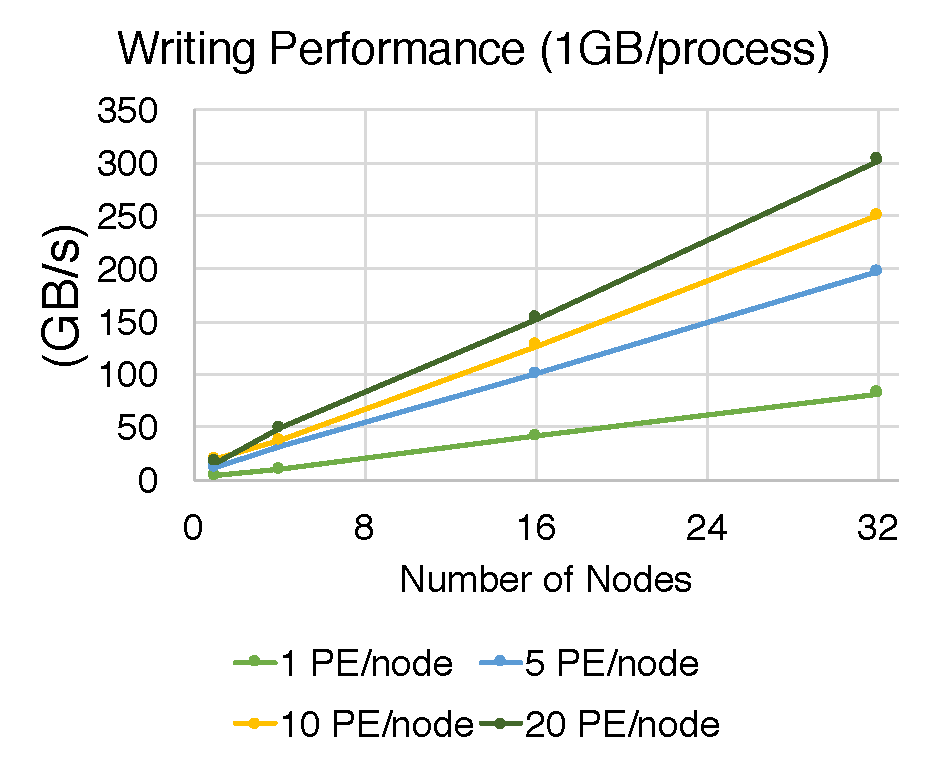
\includegraphics[width=0.45\textwidth]{figures/Adios_write_on_Summitdev.pdf}
\label{fig:summit_write}
}
\subfloat[]{
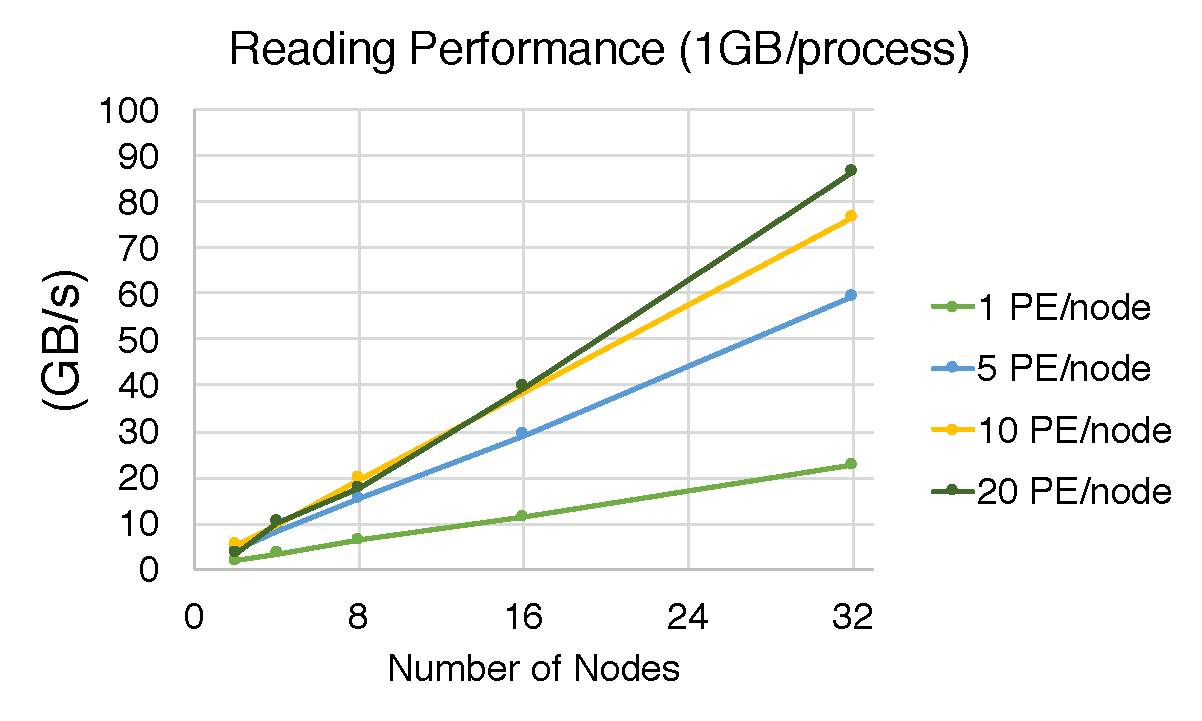
\includegraphics[width=0.45\textwidth]{figures/Adios_read_on_Summitdev.pdf}
\label{fig:summit_read}
}
\caption{ADIOS performance with Burst Buffer on Summit-dev (Summit's early access system) as of Jun 2017. Summit-dev has node-local NVMes.}
\label{fig:summit}
\end{figure}

\section{Cori@NERSC}

Unlike the node-local NVMes on Summit, the Cori system has a centralized global parallel file system built from SSDs. Any compute node has access to the whole burst buffer and therefore it is somewhat easier to use it for storing temporary data. A user can copy the data much later after the job termination to the disk based parallel file system (but before the data is purged according to NERSC policy).

\begin{wrapfigure}{l}{0.5\textwidth}
\center
%\subfloat[]{
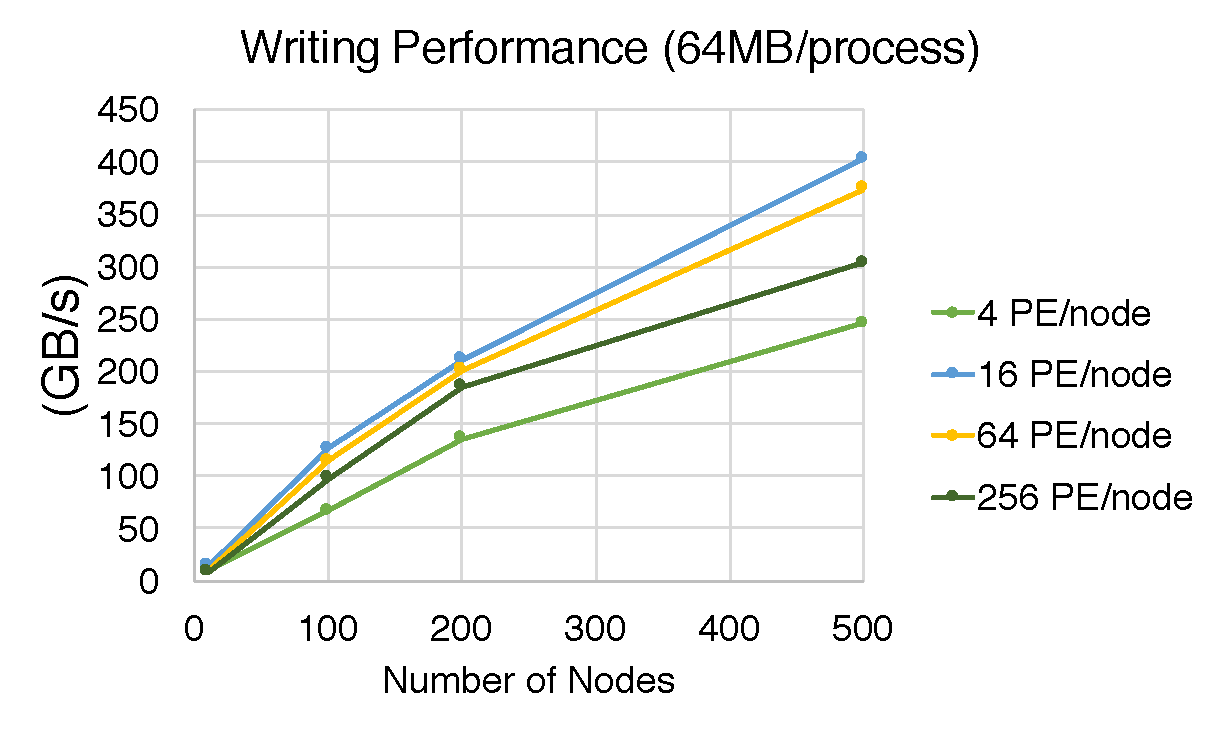
\includegraphics[width=0.45\textwidth]{figures/Adios_write_on_Cori.pdf}
%\label{fig:summit_write}
%}
\caption{ADIOS performance with Burst Buffer on Cori as of Jun 2017. Cori has a centralized global parallel file system, called Burst Buffer.}
\label{fig:cori}
\end{wrapfigure}

Here is our recommendation on how to configure ADIOS for writing to the burst buffer on Cori.
As shown in \ref{fig:cori}, we measured ADIOS writing performance on Cori's KNL nodes with POSIX method. Among different number of writers (4, 16, 64, and 256) per node, we achieved the best performance with 16 writers per node. Although there are many different factors to consider, we recommend, in general, not to use too many writers (e.g., 256 writers) or too small number of writers (e.g, 4) per node with Burst Buffer.

If you have to use full cores on KNL nodes, you may consider to use ADIOS's \verb+MPI_AGGREGATE+ transport method. With \verb+MPI_AGGREGATE+, you can control the number of writing processes with \verb+num_aggregators+ option. Also, please use \verb+striping=0+ option to use with Burst Buffer on Cori.

For an example, if you have 100 compute nodes and want maintain 16 writers per node to write to Burst Buffer on Cori, you can use the following XML code:
\begin{lstlisting}[language=XML]
<transport group="writer" 
	method="MPI_AGGREGATE">num_aggregators=1600;striping=0;</transport>
\end{lstlisting}



